\documentclass[12pt]{article}
\usepackage[margin=1in]{geometry}
\usepackage{amsmath,amsthm,amssymb,amsfonts}
\usepackage{graphicx}

\newcommand{\N}{\mathbb{N}}
\newcommand{\Z}{\mathbb{Z}}

\graphicspath{ {./} }

\newenvironment{problem}[2][Problem]{\begin{trivlist}
\item[\hskip \labelsep {\bfseries #1}\hskip \labelsep {\bfseries #2.}]}{\end{trivlist}}
%If you want to title your bold things something different just make another thing exactly like this but replace "problem" with the name of the thing you want, like theorem or lemma or whatever

\newenvironment{answer}[2][Answer]{\begin{trivlist}
\item[\hskip \labelsep {\bfseries #1}\hskip \labelsep {\bfseries #2.}]}{\end{trivlist}}

\newenvironment{warmup}[2][Warm Up]{\begin{trivlist}
\item[\hskip \labelsep {\bfseries #1}\hskip \labelsep {\bfseries #2.}]}{\end{trivlist}}

\begin{document}

%\renewcommand{\qedsymbol}{\filledbox}
%Good resources for looking up how to do stuff:
%Binary operators: http://www.access2science.com/latex/Binary.html
%General help: http://en.wikibooks.org/wiki/LaTeX/Mathematics
%Or just google stuff

\title{AST 540: Problem Set 2}
\author{Jonas Powell}
\maketitle

\begin{warmup}{1}
  In class we looked at an example of the sum of a Gaussian and a point source. Now imagine that the point source is offset from the Gaussian by a distance of three standard deviations of the Gaussian. Sketch the amplitude (only) of the FT of this new configuration. How does it compare to the FT of the Gaussian + point source when they were both centered on the same position?
\end{warmup}
\begin{answer}{Warm Up 1}
By the addition theorem, the FT of a Gaussian and a point should be the FT of a Gaussian and the FT of a point. However, the (amplitude of the) FT of a point is just a constant no matter where it is, so it should look the same.

According to the Addition Theorem for Fourier Transforms, the Fourier transform of the sum of two functions is equal to the sum of the Fourier transform of each individual function:
\begin{align*}
  FT \left( f + g \right) &= FT \left( f \right) + FT \left( g \right)
\end{align*}

Since we know that the amplitude of a Fourier transform of a point source is just a constant value (regardless of shifting, although that will affect the FT's phase), then we can add that constant to the normal Fourier transform of a Gaussian. Therefore, the amplitude of a Gaussian and a shifted point source will look the same as that Guassian and a centered point source.


\end{answer}


\bigskip
\bigskip

\begin{warmup}{2}
  Measurements of many quasars have shown that they typically have brightness temperatures of TB $\approx 10^{11}$ K and fluxes S$_{\nu} \approx$ 1 Jy. Approximately what size telescope is needed to resolve these sources? How does that compare with the size of the earth?
\end{warmup}
\begin{answer}{Warm Up 2}

We may consider the source resolved if $\Omega_{\text{antenna}} \leq \Omega_{\text{source}}$. In this case, we know that $T_A = T_B$, and so we can rearrange the equation of antenna temperature, substituting temperatures, to find the effective collecting area needed.

\begin{align*}
  T_A &= \frac{S_{\nu} \,\, A_{eff}}{2 \, k} \\
  A_{eff} &= \frac{2 \, k \, T_B}{S_{\nu}} \\
          &= 2.76 \times 10^{14} \text{  m$^2$}
\end{align*}

Rearranging to find the corresponding radius and looking up the Earth's radius, we find:
\begin{align*}
  R_{eff} &= \sqrt{\frac{A_{eff}}{\pi}} \\
          &= 9.37 \times 10^6 \text{ meters} \\
          &\approx 1.5 R_{\odot}
\end{align*}
\end{answer}



\bigskip
\bigskip

\begin{warmup}{3}
  How long would a 3 meter radio telescope with a Tsys of about 100 K have to observe Cas A to get a 10 sigma detection? Assume that the telescope is observing at 20 cm with a bandwidth of 50 MHz (and has perfect aperture efficiency), and that Cas A has a flux density of 2000 Jy at this wavelength.
\end{warmup}
\begin{answer}{Warm Up 3}

We begin with the equation characterizing noise - and consequently our standard deviation.
\begin{align*}
  \Delta T &= \frac{T_{\text{sys}}}{\sqrt{\text{B } t}} \\
           &= \sigma
\end{align*}

Since we would like a 10-$\sigma$ detection, we know that we want the antenna temperature, T$_A = 10 \sigma = 10 \Delta T$. We may find T$_A$ with our normal equation:
\begin{align*}
  T_A &= \frac{S_{\nu} A_{\text{Eff}}}{2k}
\end{align*}

We can now plug these requirements into our first equation and solve for $t$:
\begin{align*}
  T_A &= 10 \Delta T \\
      &= \frac{10 \times T_{\text{sys}}}{\sqrt{\text{B } t}} \\
  t &= \frac{1}{\text{B}} \left( \frac{20 k \times T_{\text{sys}}}{S_{\nu} A_{\text{eff}}} \right)^2 \\
    &= 4.7 \times 10^{-4} \text{ seconds}
\end{align*}

\end{answer}


\bigskip
\bigskip

\begin{warmup}{4}
  A convenient parameter for specifying the sensitivity of a radio telescope is its sensitivity in units of K/Jy; that is, the number of Kelvins of antenna temperature TA produced by an unpolarized point source whose flux density is 1 Jy.

  A) What is the effective collecting area of a radio telescope whose sensitivity is 1 K/Jy?

  B) The 2.3 GHz feed at Arecibo illuminates an elliptical aperture 225 m by 200 m in size, and the aperture efficiency over this ellipse is ηA ' 0.70. What is the sensitivity of this system in K/Jy?
\end{warmup}

\begin{answer}{Warm Up 4A}
  We can re-use the equation for effective collecting area from Warm Up 2 and simply plug in the given values:
  \begin{align*}
    A_{eff} &= 2k \,\, \frac{T_A}{S_{\nu}} \\
            &= 2k \,\, \frac{1 \text{ K}}{1 \text{ Jy}} \\
            &= 2761 \text{ m$^2$} \\
  \end{align}
\end{answer}


\bigskip
\bigskip

\begin{answer}{Warm Up 4B}
  The area of an ellipse is given by $A = \pi a b$, so we halve each given dimension to find $a$ and $b$ and find a total area of 35342 m$^2$. We may then convert that geometric area to an effective collecting area by recalling the definition of $\eta = \frac{A_{\text{eff}}}{A_{\text{geom}}}$, allowing us to find that $A_{\text{eff}} = 0.7 \times 35342 \text{ m}^2 = 24739 \text{ m}^2$

  \bigskip
  Therefore, we may find the receiver's sensitivity by:
  \begin{align*}
    \frac{T_A}{S_{\nu}} &= \frac{A_{\text{eff}}}{2 \, k} \\
                        &= 8.96 \text{ K Jy$^{-1}$}
  \end{align*}
\end{answer}


\bigskip
\bigskip

\begin{problem}{1}
  In class, we showed that a 1-D aperture with constant illumination produces a power pattern described by:

\begin{align*}
  P(\theta) \propto \text{sinc}^2 \left(\frac{ \theta D}{\lambda}\right)
\end{align*}

With D = 10 m and $\lambda = 10$ cm, use numerical techniques (e.g., using IDL, Mathematica, Python+Scipy, etc.), compute $\theta$ and P($\theta$) to at least 3 significant figures at the peaks of the first 2 sidelobes. Express them in relative terms (as a fraction of the peak of the main beam). Verify your results analytically. Turn in a copy of your code and a plot of the power pattern of the antenna with the problem set.
\end{problem}
\begin{answer}{Problem 1}
While we could solve this problem pretty easily using derivatives, we may solve it numerically with the PeakUtils Python package (see attached code). The results show sidelobe peaks at:

\begin{center}
  \begin{tabular}{ | m{5em} | m{2cm} | }
    \hline
    \theta & P(\theta) \\
    \hline
    -0.00246 & 0.01648 \\
    \hline
    -0.0014 & 0.04719 \\
    \hline
    0.00143 & 0.04719 \\
    \hline
    0.00246 & 0.01648 \\
    \hline
  \end{tabular}
\end{center}

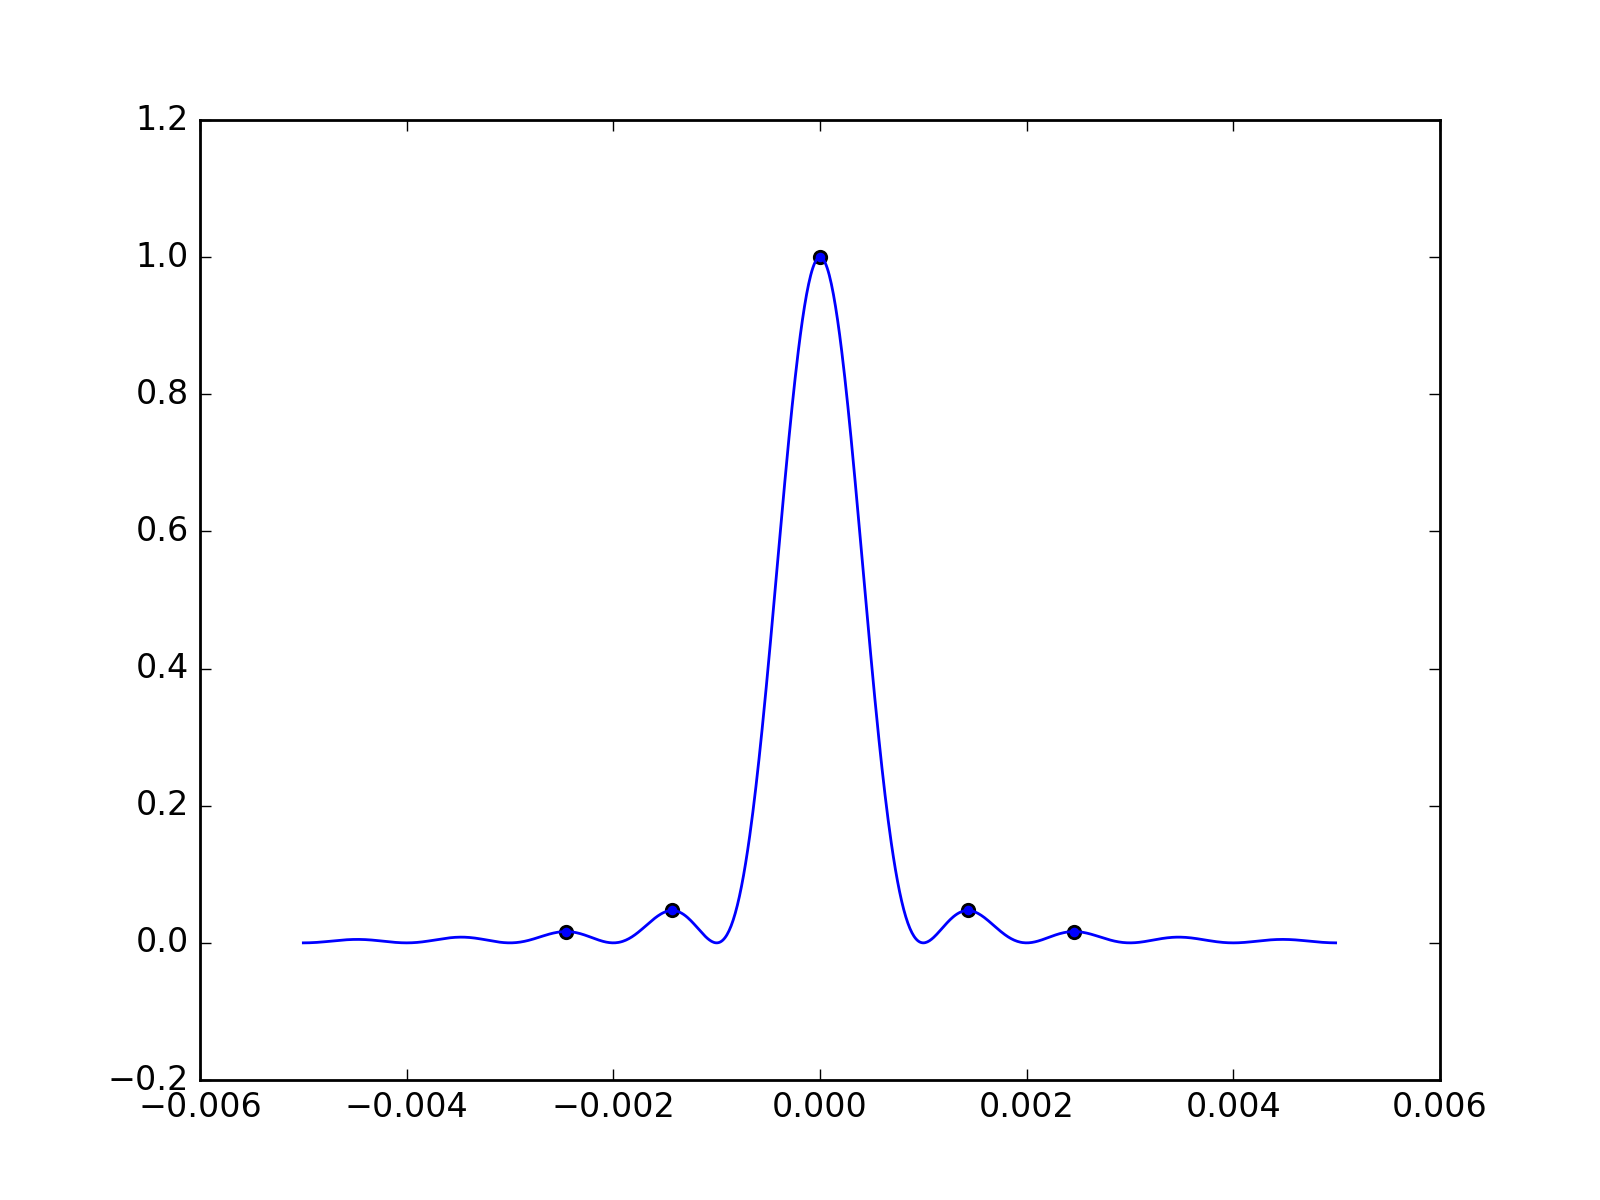
\includegraphics[scale=0.7]{problem1}


\end{answer}


\bigskip
\bigskip


\begin{problem}{2}
  A brilliant engineer named D. Donut decides that the center of a large parabolic antenna is not of much use because, for one thing, the resolution or beam size is approximately equal to $\lambda$/D, where D is the overall diameter of the antenna and λ is the wavelength. He proposes to build an antenna that is a ring section of a parabola (i.e., a parabolic reflector without the center section) with thickness $\Delta$D and diameter D $\gg \Delta$D. A special feed uniformly illuminates the reflector. He claims that the beam width will be equal to that of a normal parabolic antenna of almost twice the diameter!

  A) Estimate the gain function of this antenna, G($\theta, \phi$) (No hairy integrals, please! Just use the gain of a general aperture and assume that the ring is narrow and the aperture illumination is uniform). What is the beam width, $\theta_A$?

  B) What is the effective on-axis collecting area, A$_0$?

  C) What is the antenna beam solid angle, ΩA, using the expression that we derived in class (ΩA = $\lambda^2/A_0$)?

  D) What are the advantages and disadvantages of this antenna?

  FYI: the Culgoora Array in Australia, now defunct, consisted of a large number of paraboloid antennas arranged in a circle and had an antenna pattern something like the one discussed here.
\end{problem}

\begin{answer}{Problem 2A}
We begin by evaluating the gain function. Since our aperture illumination, $\epsilon$, is uniform, it comes out of our gain function's integral and cancels with the power term in the denominator.

\begin{align*}
  G(\theta) &= \frac{8 \pi^2}{\lambda^2} \frac{\left( \int_{D}^{D + \Delta D} \epsilon \,\, J_0 \left(\frac{2 \pi \rho \theta}{\lambda} \right) \rho \,\, d\rho \right)^2}{\int_{D}^{D + \Delta D} \epsilon^2 \, \rho \,\, d\rho}
\end{align}

Since the aperture illumination, $\epsilon$, is uniform, we may pull it out of each integral and find that they cancel. We then evaluate the remainders of each integral in the range defined by Mr. Donut and find:
\begin{align*}
  G &= \frac{2 \pi^2}{\lambda^2} J_0^2 \left( \frac{\pi D \theta}{\lambda} \right) D \, \Delta D
\end{align}

$G(\theta)$ is plotted below, with arbitrary values entered for $\lambda, D \text{, and } \Delta D$ to give us a feel for the function's form:

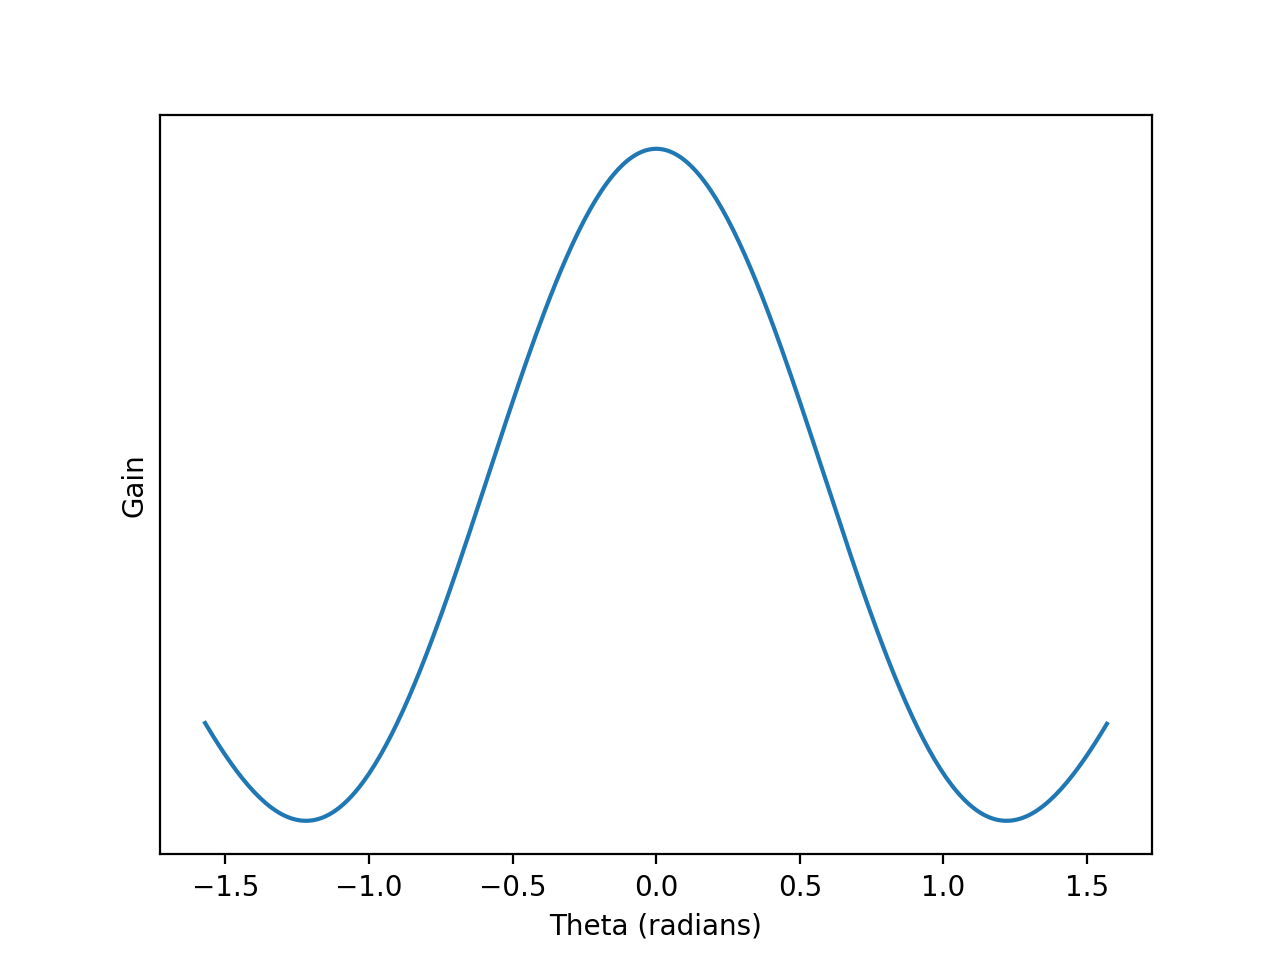
\includegraphics[scale=0.7]{problem2a}


To find the beam width, $\theta_A$, we recall that the beam width is defined to be the width of the function's main peak, it's full width half max. We find this width by setting the function $J_0^2(x) = 0.5$. Setting $x = \frac{\pi D \theta}{2\lambda}$ (doubling the $\lambda$ to capture the function's value symmetrically from 0) and solving for $\theta$, we find $\theta = 0.72 \frac{\lambda}{D}$

\end{answer}

\begin{answer}{Problem 2B}
  From class, we know that:
  \begin{align*}
    A_0 = A_{\text{eff}} = \frac{\lambda^2 G}{4 \pi}
  \end{align}

  We evaluate this at $\theta=0 \rightarrow J_0^2 = 1$:
  \begin{align*}
     A_{\text{eff}} &= \frac{\lambda^2 G}{4 \pi} \\
                    &= \frac{\lambda^2}{4 \pi} \frac{2 \pi^2 D \, \Delta D}{\lambda^2} \\
                    &= \frac{\pi}{2} D \, \Delta D
  \end{align}
\end{answer}

\begin{answer}{Problem 2C}
  \begin{align*}
    A &= \frac{\lambda^2}{A_0} \\
      &= \frac{2 \lambda^2}{\pi D \, \Delta D}
  \end{align}
\end{answer}



\bigskip
\bigskip


\begin{problem}{3}
  Qualitatively sketch the beam pattern of this aperture. Be sure to justify the components of your sketch. Use the common FT pairs and the various FT theorems we discussed in class to arrive at your result.

  Extra credit: calculate the FT of this aperture in Mathematica or the programming language of your choice (using built-in FT routines is fine; attach your code and a plot when you turn in your HW).
\end{problem}

\begin{answer}{Problem 3}
  I know this that this Fourier Transform is wrong. Ismael says it's because Python is having trouble dealing with the innately discrete formulation of my circles (each point along the circumference is a digital step), which seems reasonable, but it's frustrating that that leads to such a wrong FT image.

  \bigskip
  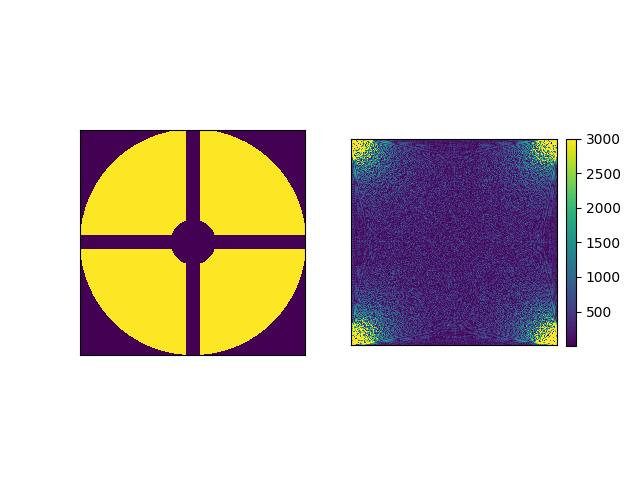
\includegraphics[scale=0.7]{problem3}
\end{answer}













\end{document}
